\documentclass[tikz]{standalone}
\usepackage{amsmath}
\definecolor{aksen}{RGB}{247,181,56}
\definecolor{bgdark}{HTML}{171D2B}
\begin{document}
\pagecolor{bgdark}
\color{white}
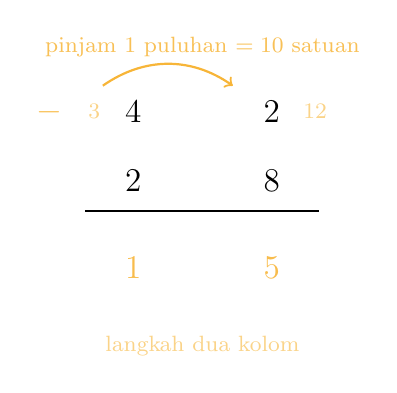
\begin{tikzpicture}[scale=1.1]
  % kolom: puluhan di kiri (x=0), satuan di kanan (x=1.6)
  \def\colX{0} \def\colY{1.6}
  \node[anchor=east, color=aksen!80] at (-0.7,3.6) {\large $-$};
  % angka
  \node at (\colX,3.6) {\large 4};   \node at (\colY,3.6) {\large 2};
  \node at (\colX,2.8) {\large 2};   \node at (\colY,2.8) {\large 8};
  \draw[thick] (-0.55,2.45) -- (2.15,2.45);
  % hasil
  \node[color=aksen!90] at (\colX,1.8) {\large 1};
  \node[color=aksen!90] at (\colY,1.8) {\large 5};
  % panah pinjam dari puluhan
  \draw[->, thick, aksen] (\colX-0.35,3.9) to[bend left=35] (\colY-0.45,3.9);
  \node[color=aksen!85, font=\footnotesize] at (0.8,4.35) {pinjam 1 puluhan $=10$ satuan};
  % coret 4 jadi 3 (digambarkan angka kecil di sampingnya)
  \node[color=aksen!60, font=\footnotesize] at (\colX-0.45,3.6) {3};
  % coret 3 jadi 13
  \node[color=aksen!60, font=\footnotesize] at (\colY+0.5,3.6) {12};
  \node[color=aksen!60, font=\footnotesize] at (0.8,0.9) {langkah dua kolom};
\end{tikzpicture}
\end{document}
